

Silver Star Mines es una empresa ficticia que opera en el sector minero, con un enfoque en la extracción y procesamiento de minerales. La compañía cuenta con una infraestructura de tecnología de la información (TI) extensa, que incluye una variedad de sistemas críticos para sus operaciones diarias. Estos sistemas son esenciales no solo para la gestión de las operaciones mineras, sino también para cumplir con las normativas de salud y seguridad que rigen la industria.

La infraestructura de TI de Silver Star Mines incluye sistemas de control de supervisión y adquisición de datos (SCADA), bases de datos que almacenan información sobre la producción y la seguridad, y servidores que gestionan las operaciones administrativas. Estos activos son vitales para el funcionamiento eficiente de la empresa y para garantizar la seguridad de los trabajadores en el sitio.

\begin{figure}[h!]
    \centering
    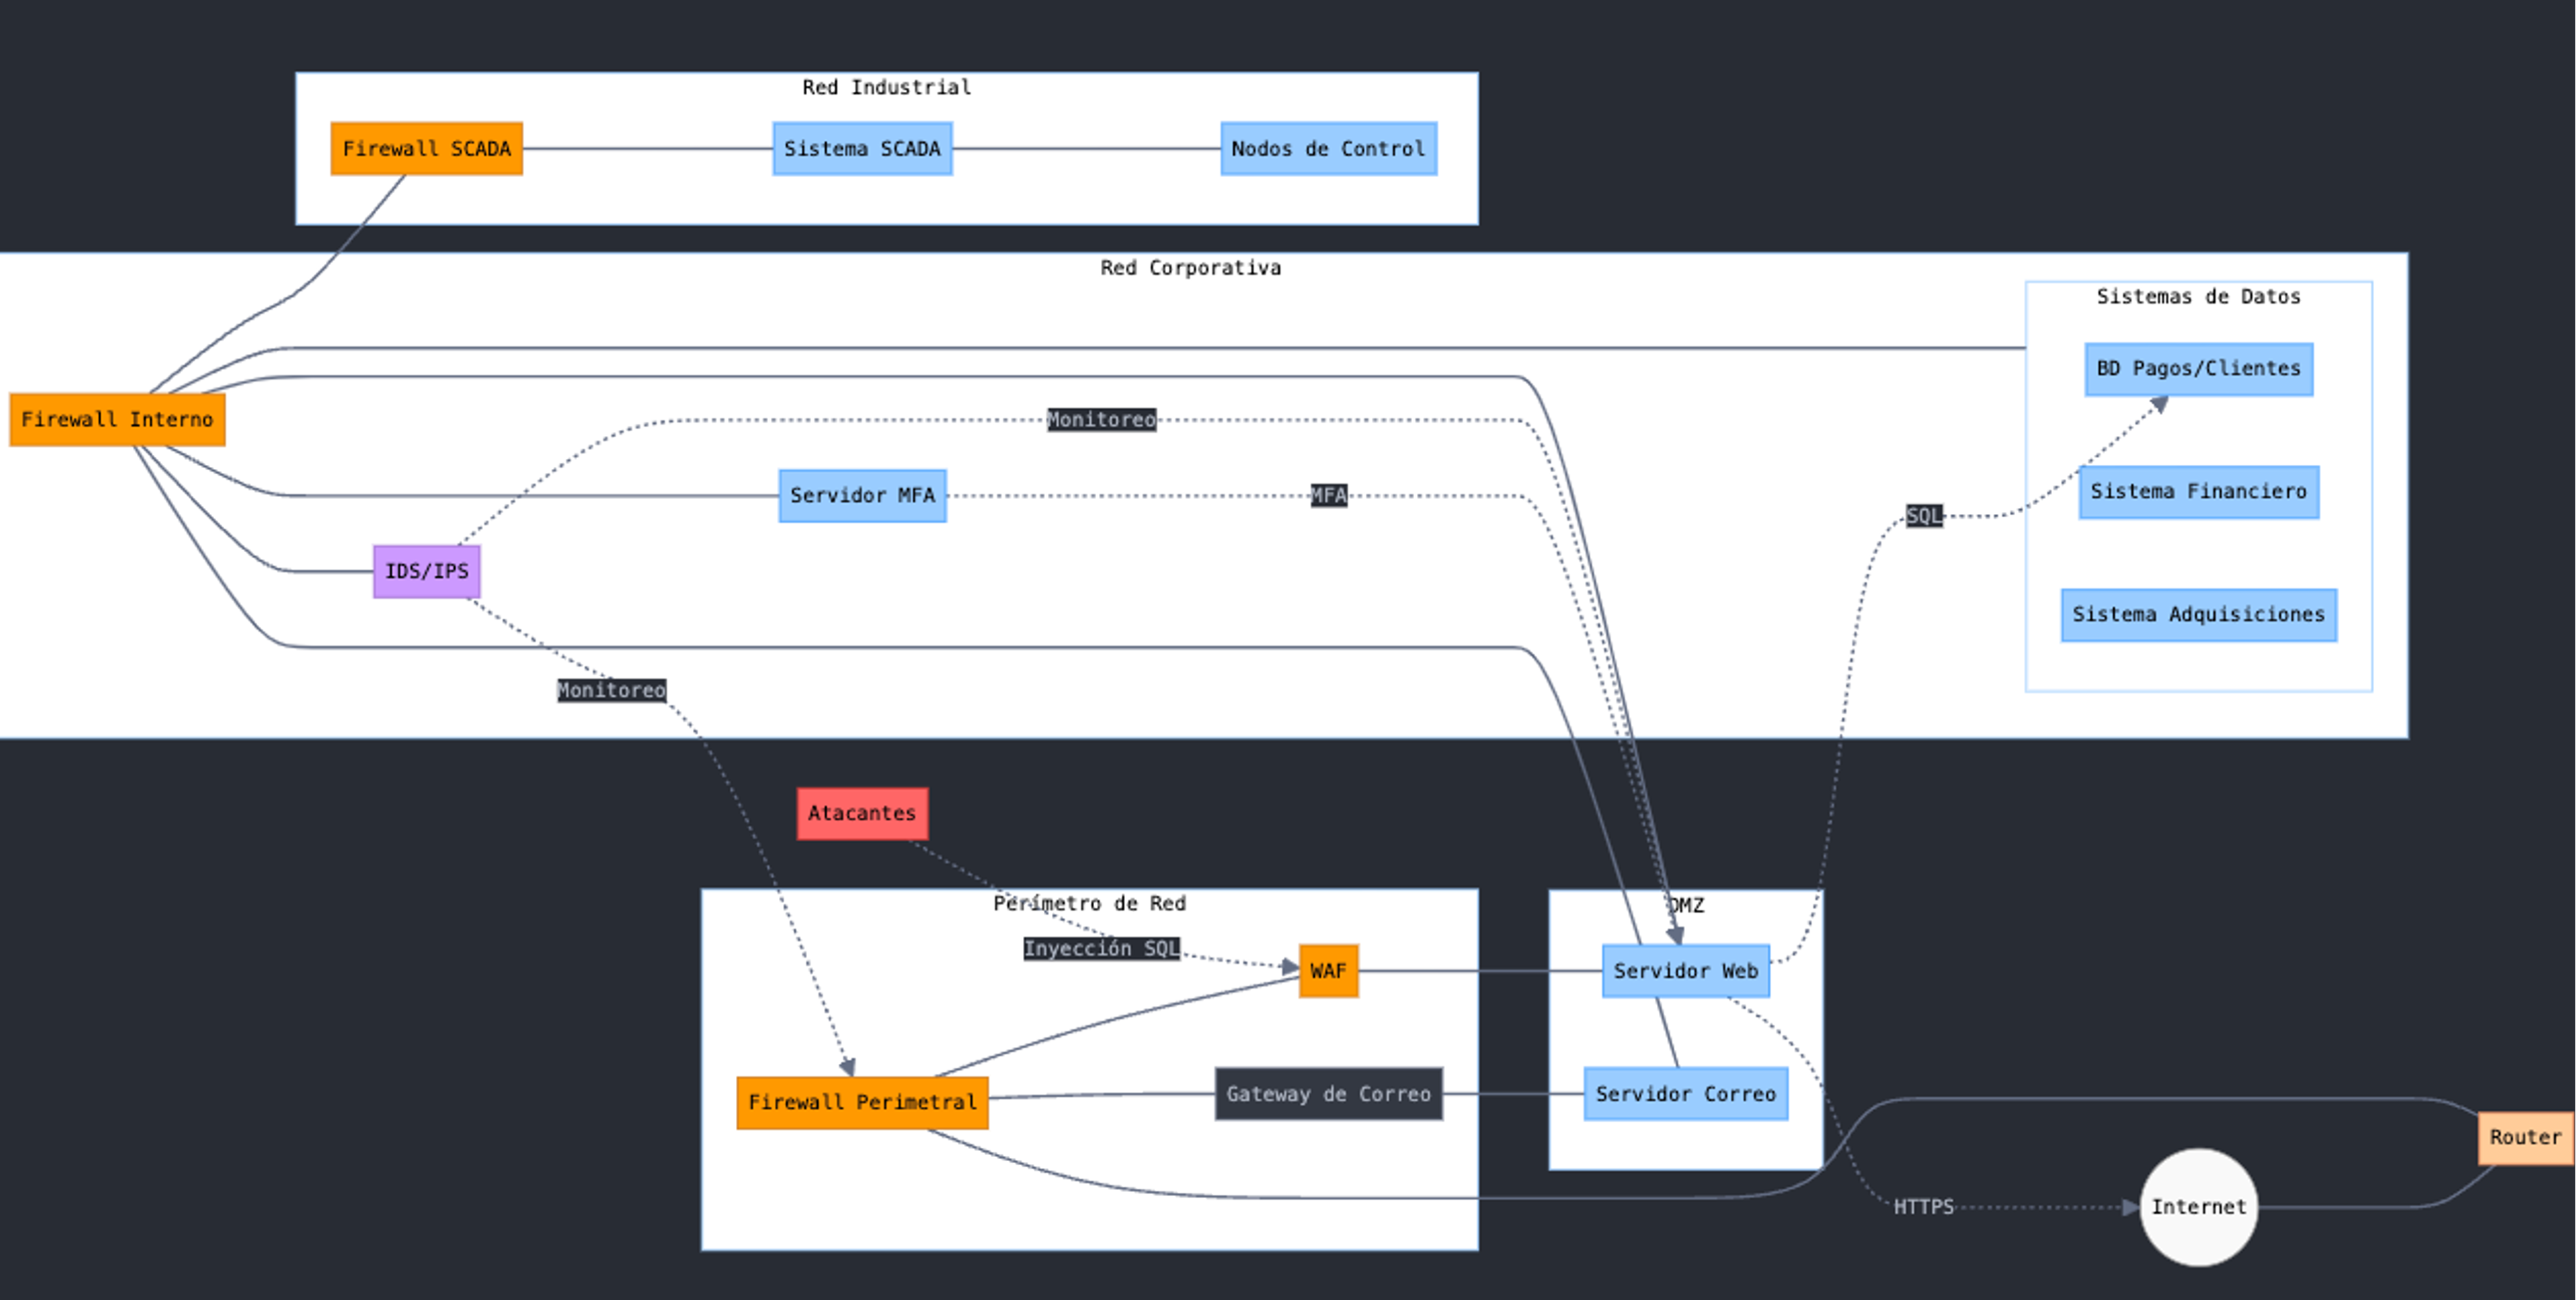
\includegraphics[width=1\linewidth]{Pictures/Imagen 1.png}
    \caption{Diagrama de Red}
    \label{fig:diagramasilverstarmines}
\end{figure}

Supongamos que un empleado de Silver Star Mines, trabajando remotamente, necesita acceder a los datos de producción. Tal como vemos en la Figura \ref{fig:diagramasilverstarmines} su solicitud viaja a través de Internet hasta llegar al \textbf{Router} principal de la empresa, el punto de entrada a toda la infraestructura de Silver Star Mines.
El router encamina esta solicitud hacia el \textbf{Firewall Perimetral}, el primer guardián de la red. Este firewall examina meticulosamente cada paquete de datos entrante para asegurarse de que cumple con las políticas de seguridad establecidas, bloqueando cualquier tráfico sospechoso o no autorizado.


Mientras tanto, un grupo de Atacantes ha estado monitoreando la red de Silver Star Mines, buscando vulnerabilidades para explotar. Intentan un ataque de inyección SQL dirigido a las aplicaciones web de la empresa. Sin embargo, el\textbf{ WAF (Firewall de Aplicaciones Web)} detecta estos patrones maliciosos en las solicitudes HTTP y los bloquea antes de que puedan alcanzar los servidores internos.

Al mismo tiempo, un proveedor envía un correo electrónico con especificaciones técnicas para un nuevo equipo de minería. Este correo pasa por el \textbf{Gateway de Correo} que filtra todos los mensajes entrantes en busca de amenazas como phishing, malware o adjuntos sospechosos, asegurando que solo los correos legítimos lleguen a los destinatarios.


Una vez que la solicitud del empleado ha sido verificada por el \textbf{firewall perimetral,} llega al \textbf{Servidor Web} ubicado en la \textbf{DMZ}. Este servidor aloja la interfaz web que permite a los empleados acceder de forma segura a ciertos datos y aplicaciones desde el exterior. Toda la comunicación se realiza a través de \textbf{HTTPS}, garantizando que los datos transmitidos estén cifrados.
Del mismo modo, el correo electrónico filtrado llega al Servidor de Correo en la DMZ, donde se almacena temporalmente antes de ser entregado a las bandejas de entrada de los destinatarios dentro de la empresa.

 
Para obtener los datos de producción solicitados, el \textbf{servidor web} necesita comunicarse con los sistemas internos de la empresa. Esta comunicación debe pasar por el \textbf{Firewall Interno}, que constituye una segunda capa de protección y controla estrictamente qué tipo de tráfico puede fluir desde la DMZ hacia la red corporativa.
Mientras estos datos atraviesan la red, el \textbf{IDS/IPS }(Sistema de Detección/Prevención de Intrusiones) monitorea constantemente todo el tráfico en busca de comportamientos anómalos o sospechosos que podrían indicar una brecha de seguridad. Este sistema funciona como un vigilante silencioso que puede alertar al equipo de seguridad ante cualquier actividad inusual.


Antes de permitir el acceso a información sensible, el \textbf{Servidor MFA} (Autenticación Multifactor) entra en acción. El empleado ya ingresó su nombre de usuario y contraseña, pero ahora debe proporcionar un segundo factor de autenticación, como un código generado en su teléfono móvil. Este sistema asegura que, incluso si las credenciales han sido comprometidas, un atacante no pueda acceder sin poseer también el dispositivo del empleado.


Con la autenticación completada exitosamente, la solicitud llega a los sistemas internos. Dependiendo de lo que necesite el empleado, podría acceder a diferentes sistemas:
\begin{itemize}
    \item El Sistema Financiero contiene toda la información contable de la empresa, incluyendo costos operativos y proyecciones financieras.
    \item El Sistema de Adquisiciones gestiona la compra de equipos, materiales y servicios necesarios para la operación minera.
    \item La BD Pagos/Clientes almacena información sobre transacciones comerciales, ventas de minerales y relaciones con los clientes.

\end{itemize}


Lo que hace especial a Silver Star Mines es su infraestructura industrial. Para acceder a los datos de producción en tiempo real, la solicitud debe atravesar otro nivel de seguridad: el \textbf{Firewall SCADA}, diseñado específicamente para proteger los sistemas de control industrial.
Una vez autorizado, el empleado puede ver la información del Sistema SCADA (Supervisión, Control y Adquisición de Datos), que monitorea y controla los procesos de extracción y procesamiento de minerales. Este sistema es crítico no solo para la eficiencia operativa, sino también para la seguridad de los trabajadores en las minas.
El SCADA se comunica constantemente con los Nodos de Control distribuidos en diferentes áreas de la mina. Estos nodos recopilan datos de sensores que miden variables como presión, temperatura, calidad del aire y niveles de producción, y también controlan equipos como bombas, ventiladores y sistemas de transporte.


Después de consultar los datos necesarios, el empleado cierra su sesión. Durante todo este proceso, la arquitectura de seguridad de Silver Star Mines ha funcionado como un conjunto de capas protectoras:

\begin{itemize}
    \item Los firewalls han controlado estrictamente el tráfico entre diferentes zonas de la red
    \item El WAF ha protegido las aplicaciones web contra ataques específicos
    \item El Gateway de Correo ha filtrado las comunicaciones entrantes
    \item El IDS ha monitoreado continuamente toda la red buscando anomalías
    \item El sistema MFA ha verificado la identidad del empleado
    \item Los firewalls especializados para SCADA han protegido la infraestructura industrial crítica

\end{itemize}


Esta arquitectura de defensa en profundidad es crucial para Silver Star Mines, ya que protege no solo la información confidencial de la empresa, sino también los sistemas físicos que controlan operaciones mineras donde la seguridad de los trabajadores depende de la integridad de estos sistemas.




\subsection{Registro de Riesgos de Silver Star Mines}




Recientemente, la dirección de Silver Star Mines ha expresado su preocupación por la creciente amenaza de ciberataques, especialmente a medida que la empresa ha conectado sus sistemas a la red corporativa para mejorar la gestión y la supervisión. Esta conexión, aunque beneficiosa, ha aumentado la exposición de los sistemas a ataques externos, lo que plantea un riesgo significativo para la integridad y disponibilidad de los datos.

La empresa se enfrenta a varios riesgos, incluyendo:
\begin{itemize}
    \item \textbf{Compromiso no autorizado de los sistemas SCADA}: Dado que estos sistemas son críticos para la operación segura de las minas, un ataque exitoso podría tener consecuencias graves, incluyendo daños a la infraestructura y riesgos para la seguridad de los empleados.
    \item \textbf{Robo de datos}: La integridad de la información almacenada en bases de datos es esencial para la toma de decisiones. Un ataque que comprometa esta información podría resultar en pérdidas financieras y daños a la reputación de la empresa.
    \item ...
\end{itemize}

A continuación, se presenta una tabla que resume los riesgos identificados en Silver Star Mines, junto con su probabilidad, consecuencias y nivel de riesgo.

\begin{table}[h]
    \centering
    \caption{Registro de Riesgos de Silver Star Mines}
    \begin{tabularx}{\textwidth}{@{}X X X X X X@{}}
        \toprule
        \textbf{Activo} & \textbf{Amenaza/Vul.} & \textbf{Control Existente} & \textbf{Prob.} & \textbf{Consec.} & \textbf{Nivel de Riesgo} \\ \midrule
        Fiabilidad e integridad de los nodos SCADA & Compromiso no autorizado & Firewalls en capas & Rara & Mayor & Alto \\ \hline
        Integridad de la información almacenada & Robo de datos & Políticas de seguridad & Posible & Mayor & Extremo \\ \hline
        Disponibilidad del sistema financiero & Ataques de red & Firewalls, políticas & Posible & Moderado & Alto \\ \hline
        Disponibilidad del sistema de adquisiciones & Ataques de red & Firewalls, políticas & Posible & Moderado & Alto \\ \hline
        Disponibilidad del sistema de mantenimiento & Ataques de red & Firewalls, políticas & Posible & Menor & Medio \\ \hline
        Disponibilidad, integridad y confidencialidad de los servicios de correo & Ataques de red & Firewalls, gateway de correo & Casi Cierto & Menor & Alto \\ \bottomrule
    \end{tabularx}
\end{table}
PD: Un \textbf{gateway} (puerta de enlace) es un dispositivo que actúa como un punto de acceso entre dos redes diferentes, permitiendo la comunicación y el intercambio de datos entre ellas. En el contexto de la seguridad informática, un gateway puede incluir funciones de filtrado y monitoreo de tráfico, ayudando a proteger la red interna de amenazas externas. Por ejemplo, un gateway de correo puede filtrar correos electrónicos entrantes para detectar y bloquear spam o malware antes de que lleguen a los servidores internos.



\section{Caso:  Ataque DDoS}

\begin{tcolorbox}[colback=gray!5!white,colframe=orange!60!gray,title=caso 1]
\textbf{Antes del ataque}: un grupo de estudiantes universitarios creó una botnet con la intención de atacar varios servidores y redes de juegos. Una botnet es un conjunto de computadoras infectadas por malware que están bajo el control de un único actor de amenaza, conocido como ``bot-herder''. Cada computadora en la botnet se puede controlar de forma remota para enviar un paquete de datos a un sistema de destino. En un ataque de botnet, los ciberdelincuentes instruyen a todos los bots de la botnet a enviar paquetes de datos al sistema objetivo al mismo tiempo, lo que resulta en un ataque DDoS.
%
El grupo de estudiantes universitarios publicó el código de la botnet en línea para que fuera accesible a miles de usuarios de Internet y las autoridades no pudieran rastrear la botnet hasta los estudiantes. Al hacerlo, hicieron posible que otros actores maliciosos aprendieran el código de la botnet y lo controlaran de forma remota. 

\textbf{El día del ataque}
A las 7:00 am del día del ataque, la botnet envió decenas de millones de solicitudes de DNS al proveedor de servicios. Esto abrumó el sistema y el servicio DNS se cerró. Esto significaba que no se podía acceder a todos los sitios web que utilizaban el proveedor de servicios. Cuando los usuarios intentaron acceder a varios sitios web, no fueron dirigidos al sitio web que escribieron en su navegador. Se produjeron interrupciones en cada servicio en toda América del Norte y Europa. \\ \textbf{Referencia}: \url{https://www.welivesecurity.com/la-es/2016/10/26/ataques-ddos-a-la-iot-octubre/} 
\end{tcolorbox}

hint: \textit{servidores DNS traducen los nombres de dominio de los sitios web a la dirección IP del sistema que contiene la información del sitio web. Por ejemplo, si un usuario escribiera la URL de un sitio web, un servidor DNS la traduciría en una dirección IP numérica que dirige el tráfico de la red a la ubicación del servidor del sitio web.}


%\textbf{Ejercicio: buscar la IP de uai.cl - escribirla en el navegador - chequear que suceda lo descrito.}



